% CS615 Aspects of System Administration
% Author: Jan Schaumann <jschauma@netmeister.org>
% $Id: slides.tex,v 1.3 2005/01/24 03:39:55 jschauma Exp $

\documentclass[xga]{xdvislides}
\usepackage[landscape]{geometry}
\usepackage{graphics}
\usepackage{graphicx}
\usepackage{colordvi}

\begin{document}
\setfontphv

%%% Headers and footers
\lhead{\slidetitle}				% default:\lhead{\slidetitle}
\chead{CS615 - Aspects of System Administration}% default:\chead{\relax}
\rhead{Slide \thepage}				% default:\rhead{\sectiontitle}
\lfoot{\Gray{Lecture 01: Introduction}}		% default:\lfoot{\slideauthor}
\cfoot{\relax}					% default:\cfoot{\relax}
\rfoot{\Gray{\today}}

\vspace*{\fill}
\begin{center}
	\Hugesize
		CS615 - Aspects of System Administration\\ [1em]
	\hspace*{5mm}\blueline\\ [1em]
	\Normalsize
		Department of Computer Science\\
		Stevens Institute of Technology\\
		Jan Schaumann\\
		\verb+jschauma@cs.stevens.edu+ \\
		\verb+http://www.cs.stevens.edu/~jschauma/615/+
\end{center}
\vspace*{\fill}

\subsection{First: a volunteer, please!}
\vspace*{\fill}
\Huge
\begin{center}
Collaborative Glossary Collector \\
collect acronyms in each class
\end{center}
\Normalsize
\vspace*{\fill}

\subsection{A typical System Administrator}
\vspace*{\fill}
\begin{figure}[hb]
	\begin{center}
		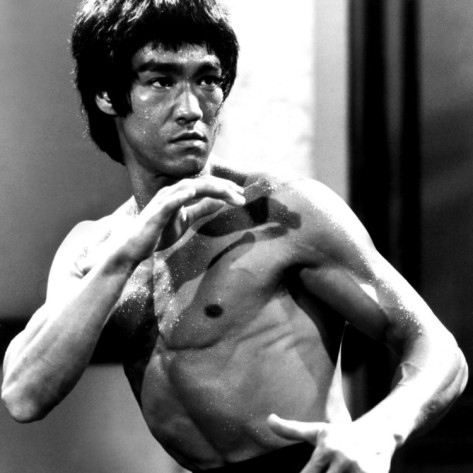
\includegraphics[scale=0.6]{pics/enter-the-dragon.eps} \\
		
\includegraphics[scale=0.2]{pics/little-dragon.eps} \\
	\end{center}
\end{figure}
\vspace*{\fill}

\subsection{Happy Chinese New Year!}
\vspace*{\fill}
\begin{figure}[hb]
	\begin{center}
		
\includegraphics[scale=0.4]{pics/may-you-realize-your-ambitions.eps} \\
	\end{center}
\end{figure}
\vspace*{\fill}




\subsection{The Job of a System Administrator}
What {\bf exactly} does a {\em System Administrator} do?

\subsection{The Job of a System Administrator}
\begin{figure}[hb]
	\begin{center}
		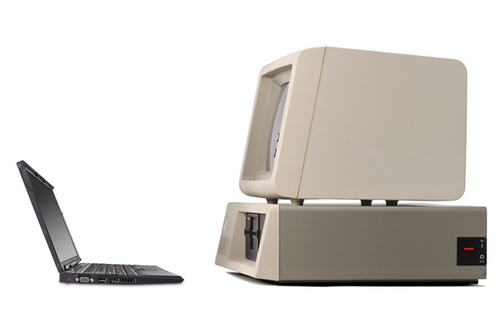
\includegraphics[scale=0.9]{pics/computers.eps} \\
	\end{center}
\end{figure}

\subsection{The Job of a System Administrator}
\vspace*{\fill}
\begin{figure}[hb]
	\begin{center}
		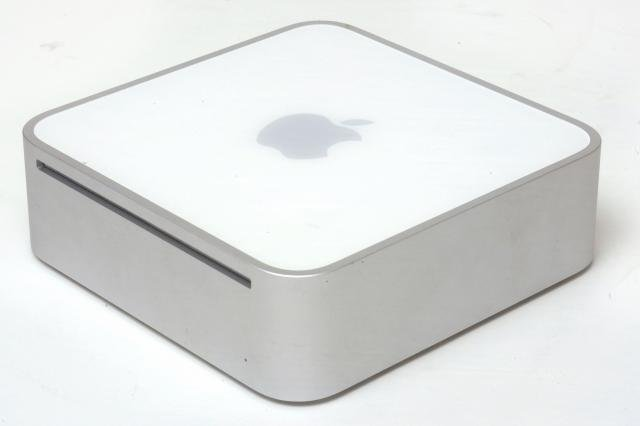
\includegraphics[scale=0.6]{pics/macmini.eps} \\
	\end{center}
\end{figure}
\vspace*{\fill}

\subsection{The Job of a System Administrator}
\vspace*{\fill}
\begin{figure}[hb]
	\begin{center}
		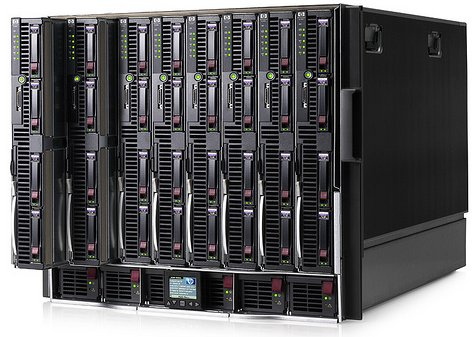
\includegraphics[scale=1.0]{pics/blades.eps} \\
	\end{center}
\end{figure}
\vspace*{\fill}

\subsection{The Job of a System Administrator}
\vspace*{\fill}
\begin{figure}[hb]
	\begin{center}
		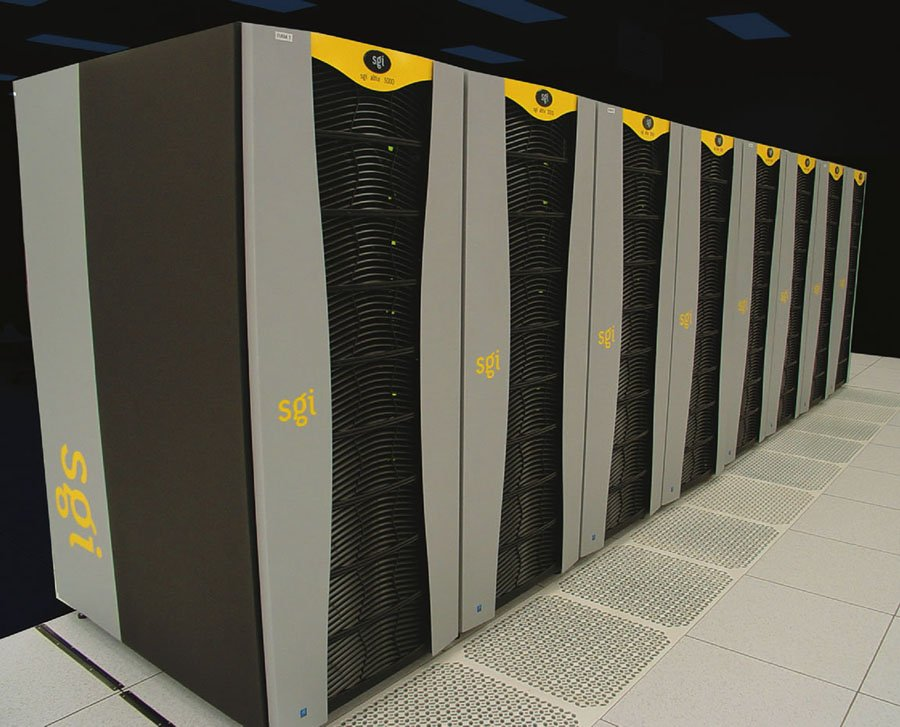
\includegraphics[scale=0.4]{pics/altix.eps} \\
	\end{center}
\end{figure}
\vspace*{\fill}

\subsection{The Job of a System Administrator}
\vspace*{\fill}
\begin{figure}[hb]
	\begin{center}
		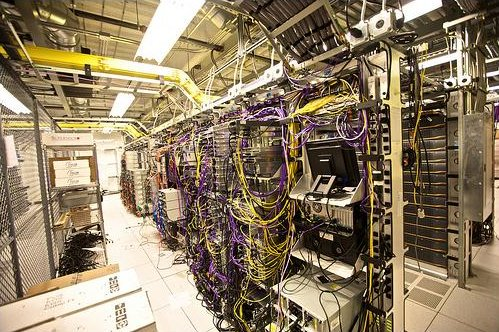
\includegraphics[scale=0.8]{pics/datacenter.eps} \\
	\end{center}
\end{figure}
\vspace*{\fill}

\subsection{The Job of a System Administrator}
\vspace*{\fill}
\begin{figure}[hb]
	\begin{center}
		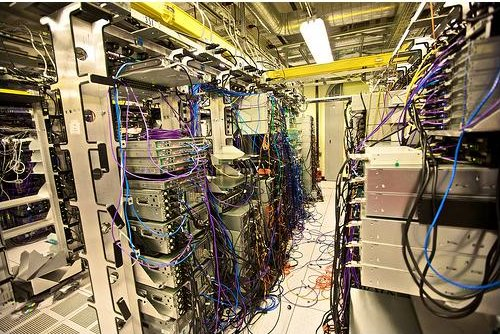
\includegraphics[scale=0.8]{pics/datacenter2.eps} \\
	\end{center}
\end{figure}
\vspace*{\fill}



\subsection{The Job of a System Administrator}
\vspace*{\fill}
\begin{figure}[hb]
	\begin{center}
		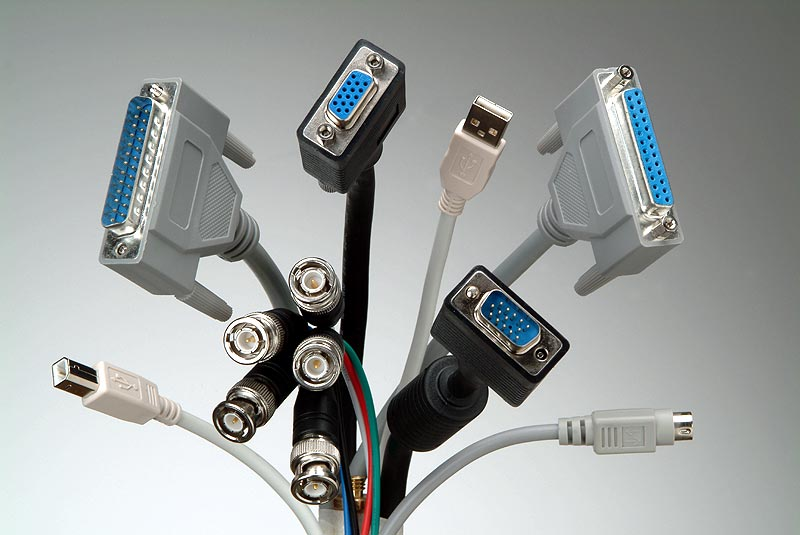
\includegraphics[scale=0.7]{pics/computer-cables-big.eps} \\
	\end{center}
\end{figure}
\vspace*{\fill}

\subsection{The Job of a System Administrator}
\vspace*{\fill}
\begin{figure}[hb]
	\begin{center}
		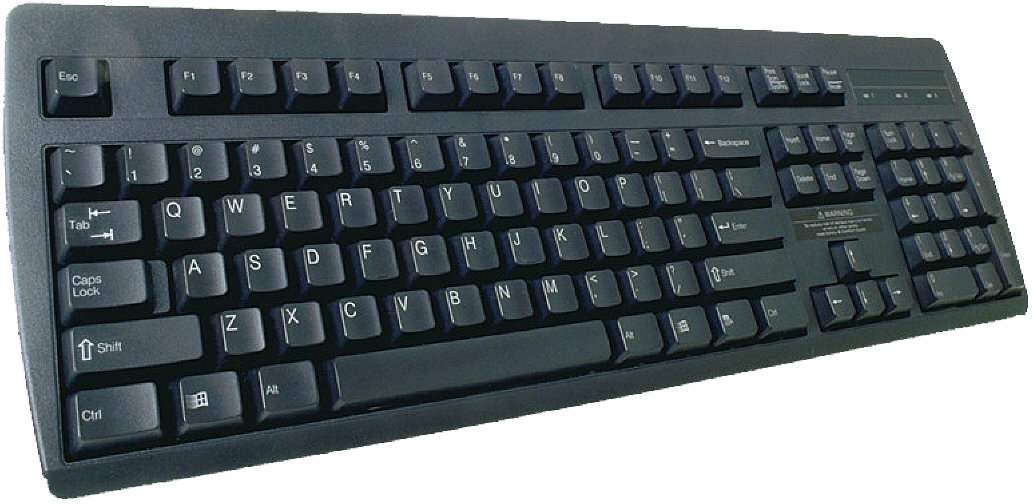
\includegraphics[scale=4.0]{pics/keyboard.eps} \\
	\end{center}
\end{figure}
\vspace*{\fill}

\subsection{The Job of a System Administrator}
\vspace*{\fill}
\begin{figure}[hb]
	\begin{center}
		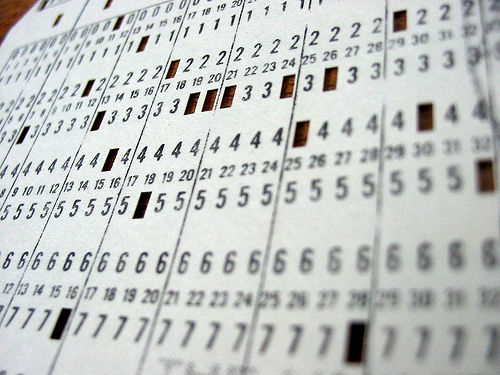
\includegraphics[scale=0.7]{pics/punchcard.eps} \\
	\end{center}
\end{figure}
\vspace*{\fill}

\subsection{The Job of a System Administrator}
\vspace*{\fill}
\begin{figure}[hb]
	\begin{center}
		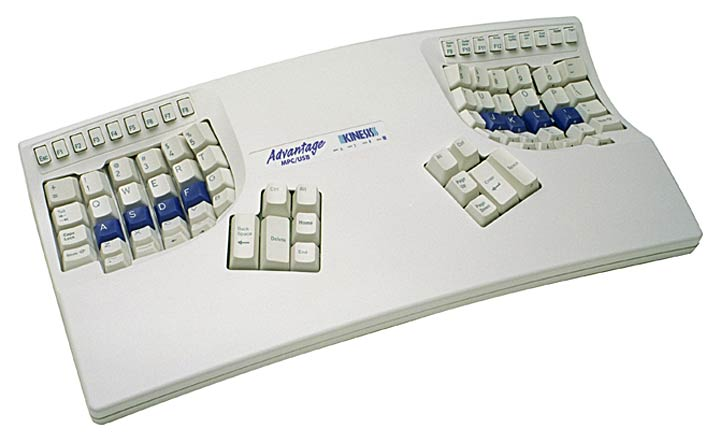
\includegraphics[scale=0.9]{pics/kinesis.eps} \\
	\end{center}
\end{figure}
\vspace*{\fill}

\subsection{The Job of a System Administrator}
\vspace*{\fill}
\begin{figure}[hb]
	\begin{center}
		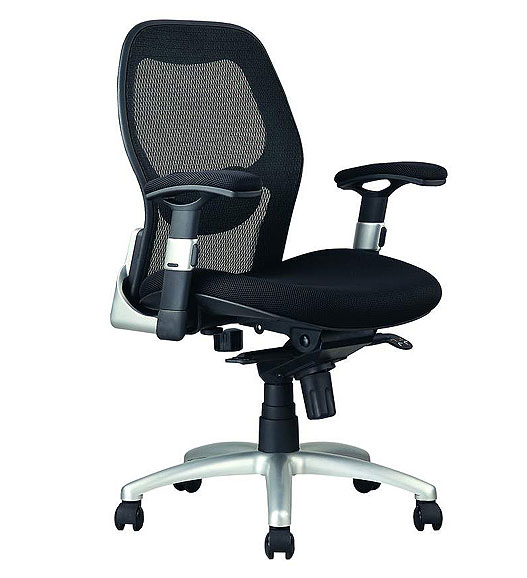
\includegraphics[scale=0.65]{pics/office-chair.eps} \\
	\end{center}
\end{figure}
\vspace*{\fill}

\subsection{The Job of a System Administrator}
\vspace*{\fill}
\begin{figure}[hb]
	\begin{center}
		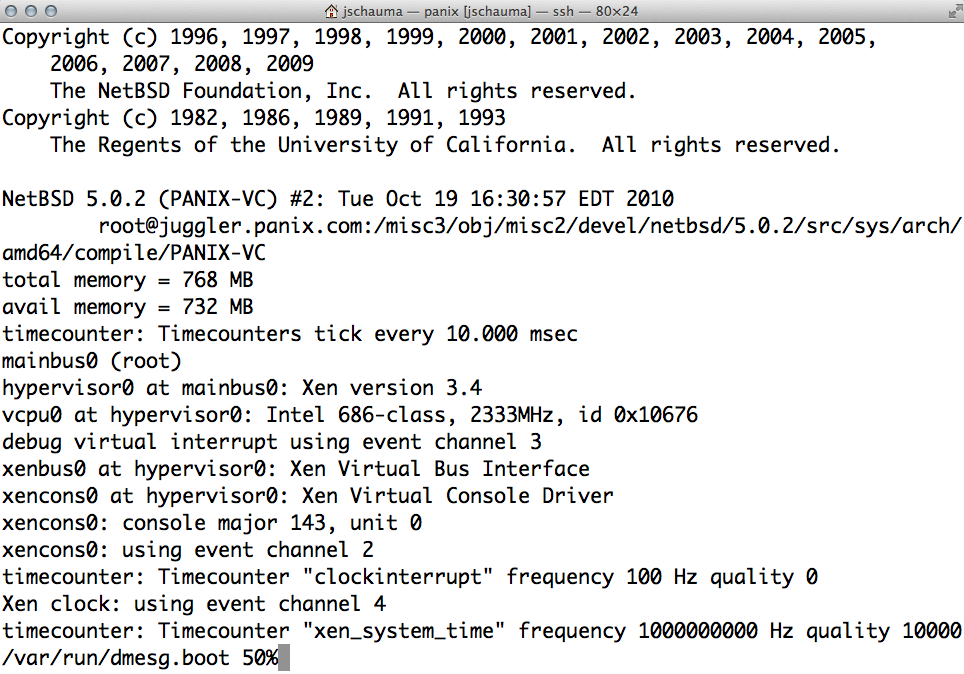
\includegraphics[scale=0.4]{pics/dmesg.eps} \\
	\end{center}
\end{figure}
\vspace*{\fill}

\subsection{The Job of a System Administrator}
\vspace*{\fill}
\begin{figure}[hb]
	\begin{center}
		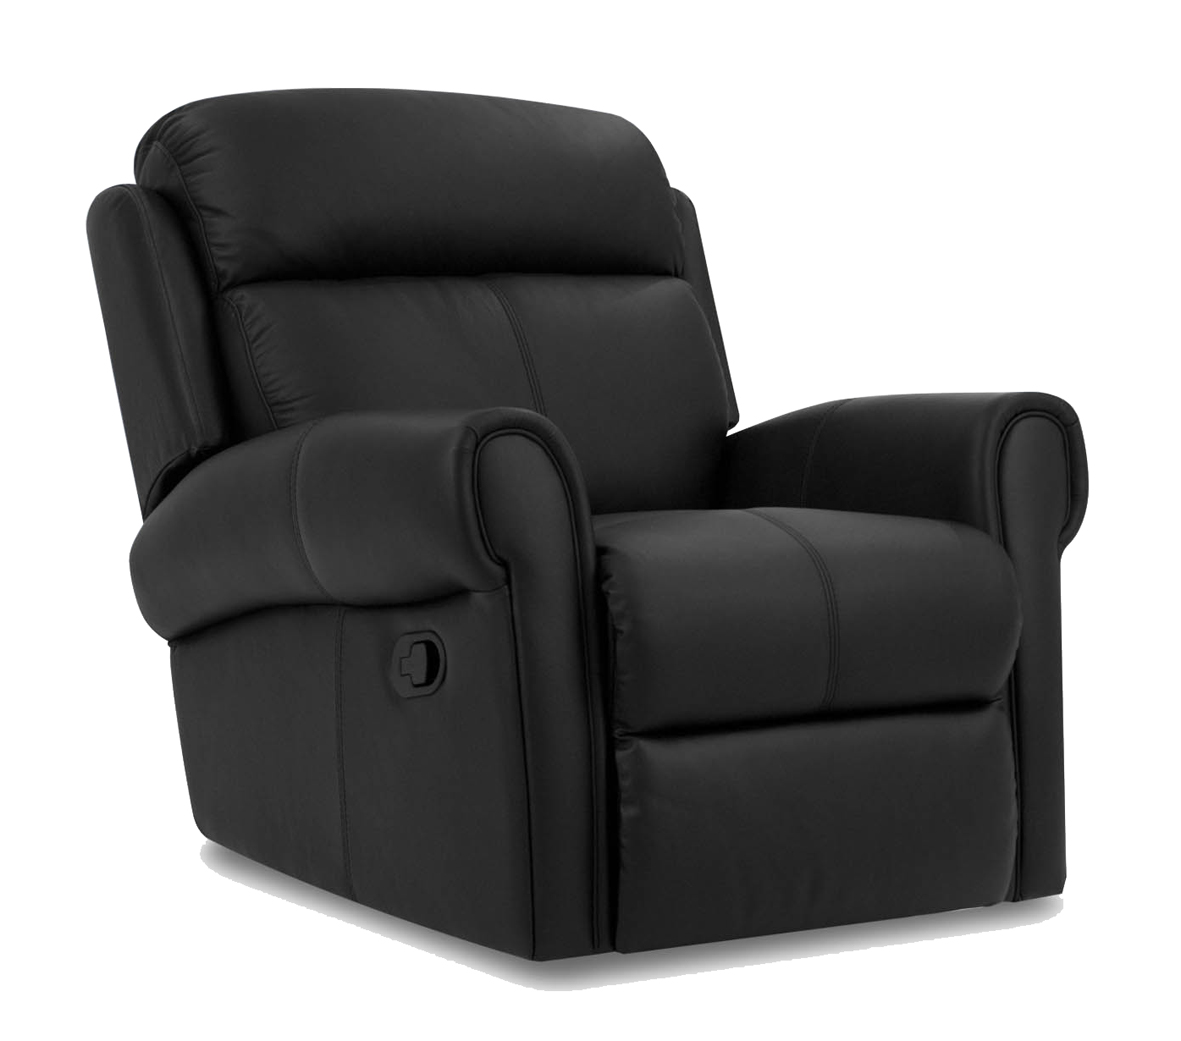
\includegraphics[scale=1.1]{pics/armchair.eps} \\
	\end{center}
\end{figure}
\vspace*{\fill}

\subsection{The Job of a System Administrator}
\vspace*{\fill}
\begin{figure}[hb]
	\begin{center}
		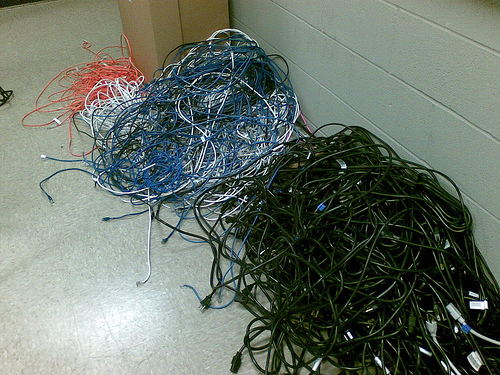
\includegraphics[scale=0.7]{pics/cable-mess.eps} \\
	\end{center}
\end{figure}
\vspace*{\fill}

\subsection{The Job of a System Administrator}
\vspace*{\fill}
\begin{figure}[hb]
	\begin{center}
		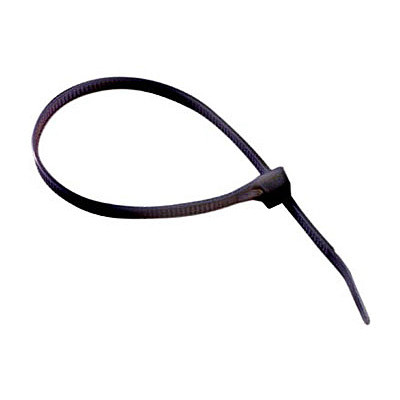
\includegraphics[scale=0.7]{pics/Cable_Tie.eps} \\
	\end{center}
\end{figure}
\vspace*{\fill}

\subsection{The Job of a System Administrator}
\vspace*{\fill}
\begin{figure}[hb]
	\begin{center}
		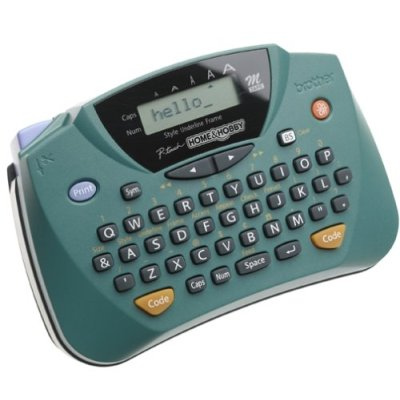
\includegraphics[scale=0.7]{pics/labelmaker.eps} \\
	\end{center}
\end{figure}
\vspace*{\fill}

\subsection{The Job of a System Administrator}
\vspace*{\fill}
\begin{figure}[hb]
	\begin{center}
		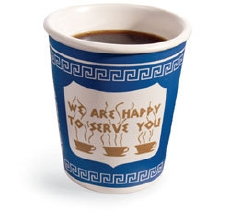
\includegraphics[scale=1.2]{pics/coffee.eps} \\
	\end{center}
\end{figure}
\vspace*{\fill}

\subsection{The Job of a System Administrator}
\vspace*{\fill}
\begin{figure}[hb]
	\begin{center}
		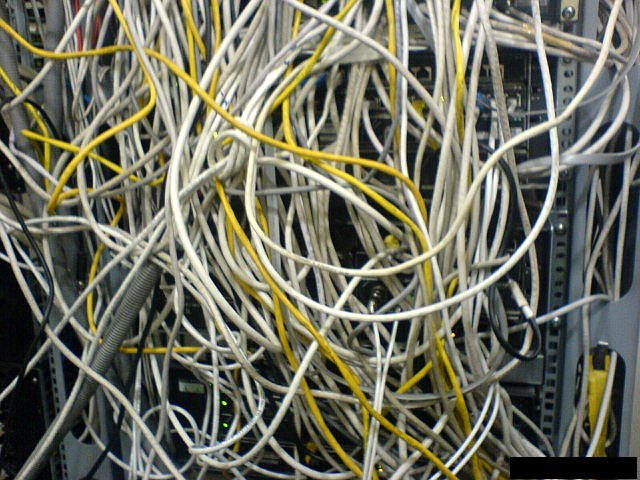
\includegraphics[scale=0.6]{pics/cable_mess.eps} \\
	\end{center}
\end{figure}
\vspace*{\fill}

\subsection{The Job of a System Administrator}
\vspace*{\fill}
\begin{figure}[hb]
	\begin{center}
		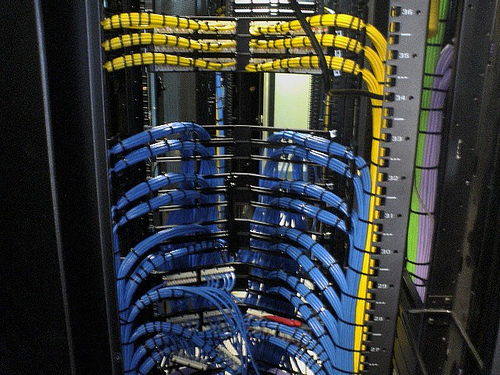
\includegraphics[scale=0.7]{pics/cables2.eps} \\
	\end{center}
\end{figure}
\vspace*{\fill}

\subsection{The Job of a System Administrator}
\vspace*{\fill}
\begin{figure}[hb]
	\begin{center}
		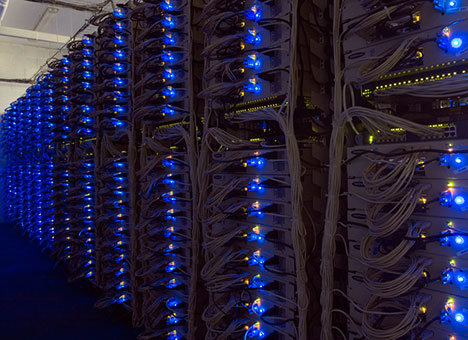
\includegraphics[scale=1.1]{pics/data-center-servers-t001.eps} \\
	\end{center}
\end{figure}
\vspace*{\fill}

\subsection{The Job of a System Administrator}
\vspace*{\fill}
\begin{figure}[hb]
	\begin{center}
		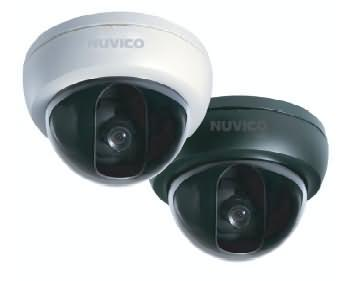
\includegraphics[scale=0.9]{pics/camera.eps} \\
	\end{center}
\end{figure}
\vspace*{\fill}

\subsection{The Job of a System Administrator}
\vspace*{\fill}
\begin{figure}[hb]
	\begin{center}
		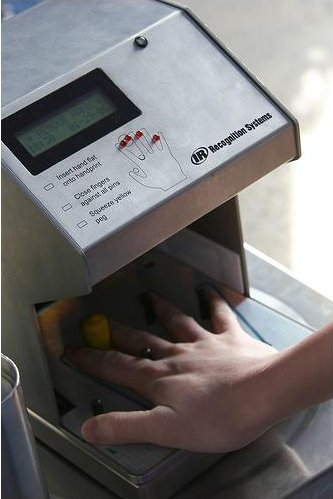
\includegraphics[scale=0.5]{pics/hand-scanner.eps} \\
	\end{center}
\end{figure}
\vspace*{\fill}


\subsection{The Job of a System Administrator}
\vspace*{\fill}
\begin{center}
	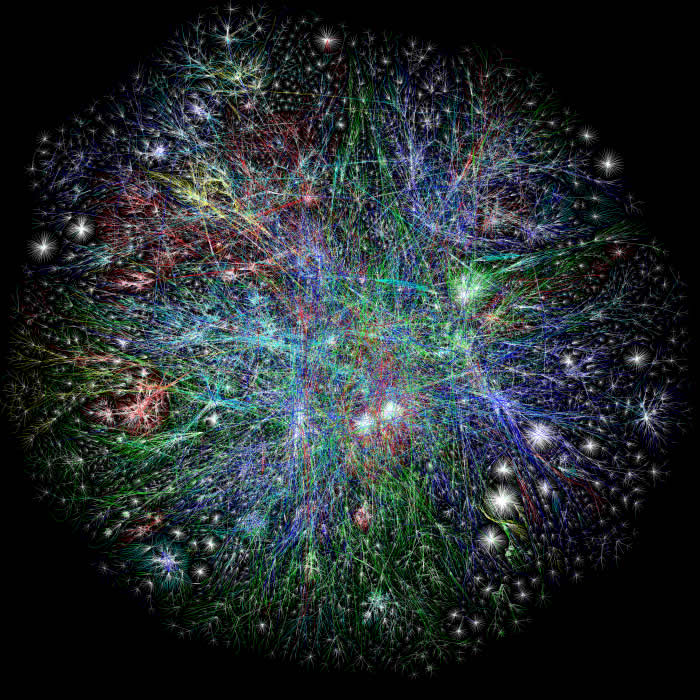
\includegraphics[scale=0.3]{pics/internet.eps} \\
	\small
	{\tt http://www.opte.org/maps/}
	\Normalsize
\end{center}
\vspace*{\fill}

\subsection{The Job of a System Administrator}
\vspace*{\fill}
\begin{figure}[hb]
	\begin{center}
		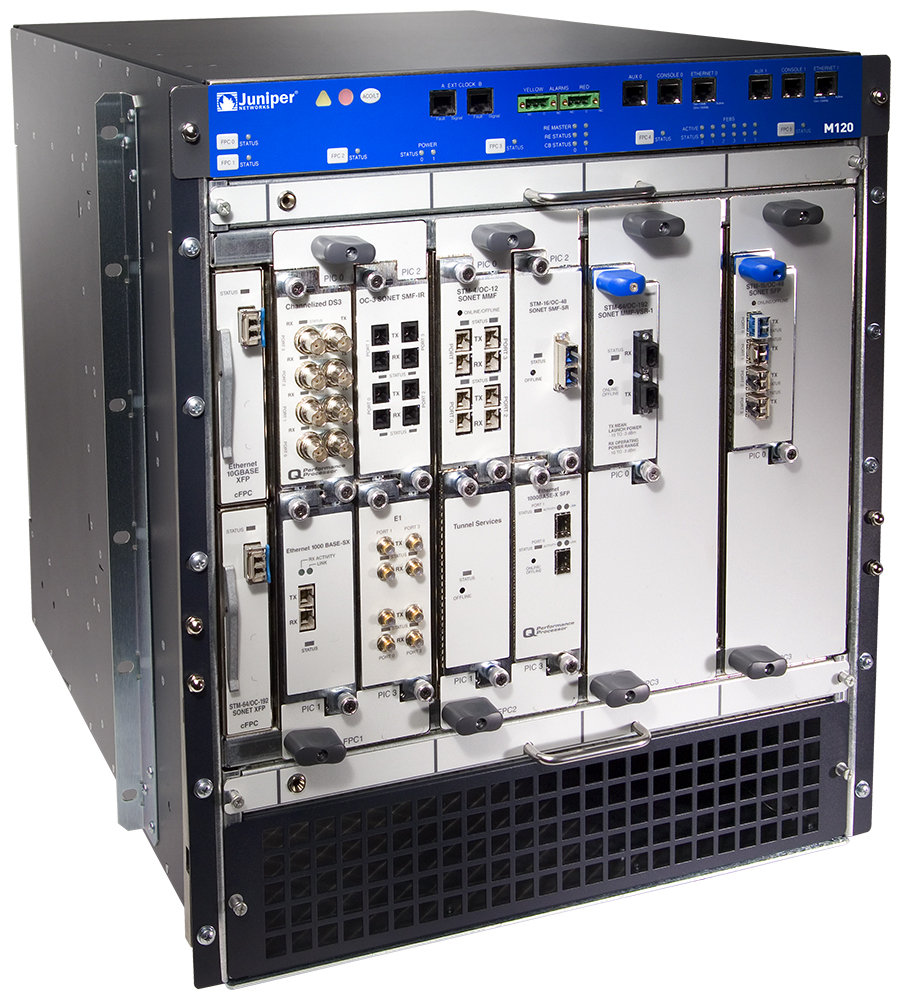
\includegraphics[scale=0.4]{pics/juniper.eps} \\
	\end{center}
\end{figure}
\vspace*{\fill}

\subsection{The Job of a System Administrator}
\vspace*{\fill}
\begin{figure}[hb]
	\begin{center}
		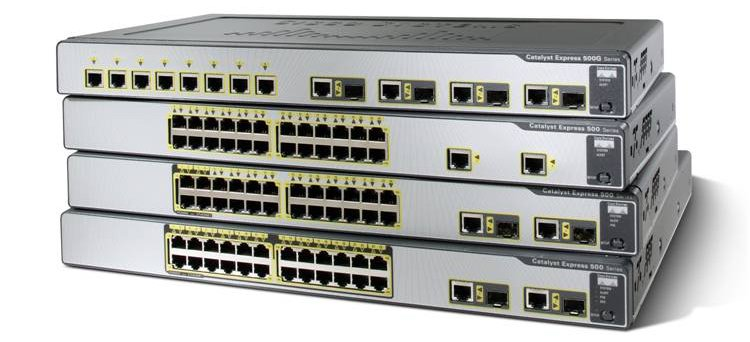
\includegraphics[scale=1.6]{pics/switches.eps} \\
	\end{center}
\end{figure}
\vspace*{\fill}

\subsection{The Job of a System Administrator}
\vspace*{\fill}
\begin{figure}[hb]
	\begin{center}
		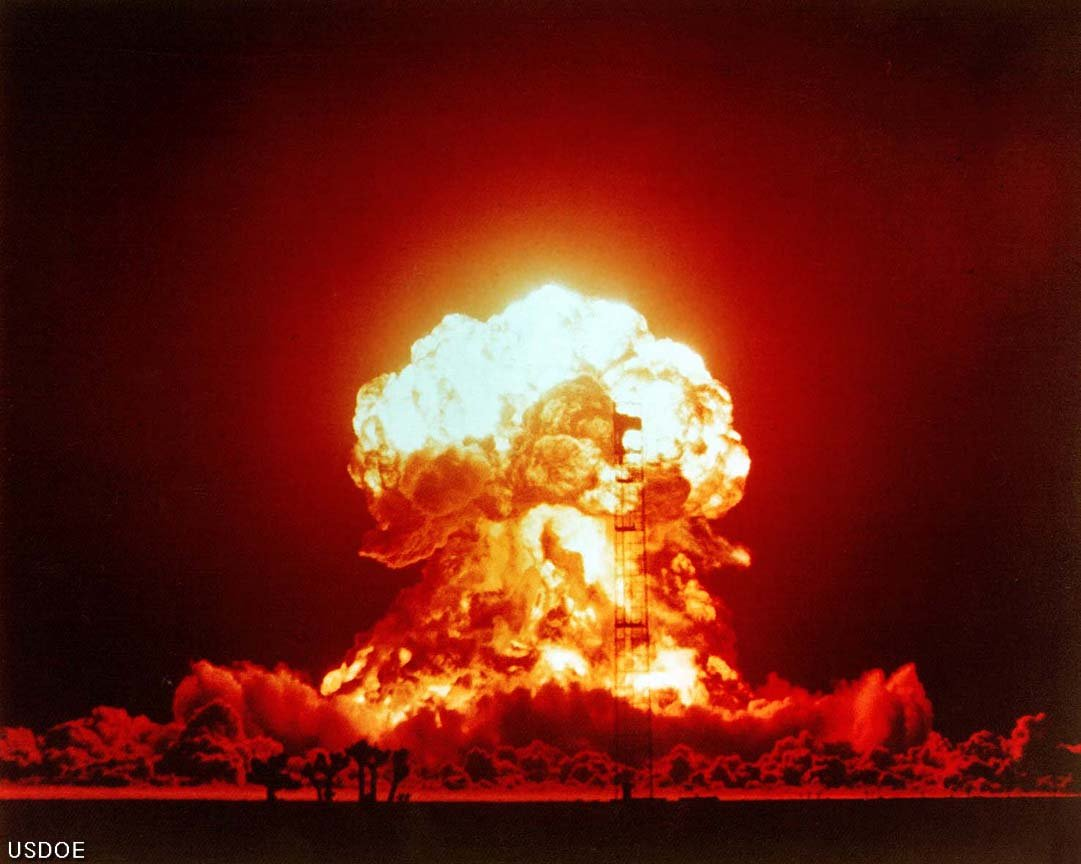
\includegraphics[scale=0.3]{pics/mushroom_cloud.eps} \\
	\end{center}
\end{figure}
\vspace*{\fill}

\subsection{The Job of a System Administrator}
\vspace*{\fill}
\begin{figure}[hb]
	\begin{center}
		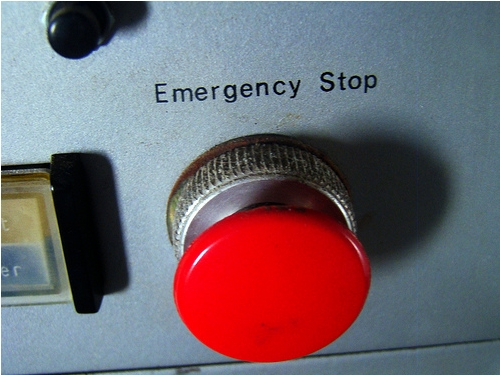
\includegraphics[scale=0.75]{pics/big-red-button.eps} \\
	\end{center}
\end{figure}
\vspace*{\fill}

\subsection{The Job of a System Administrator}
\vspace*{\fill}
\begin{figure}[hb]
	\begin{center}
		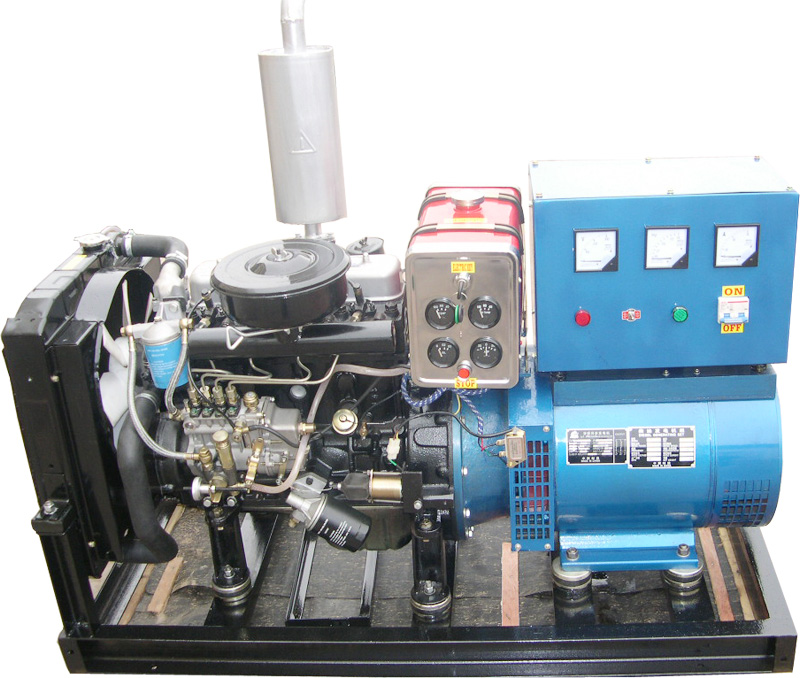
\includegraphics[scale=1.8]{pics/diesel-generator.eps} \\
	\end{center}
\end{figure}
\vspace*{\fill}

\subsection{The Job of a System Administrator}
\vspace*{\fill}
\begin{figure}[hb]
	\begin{center}
		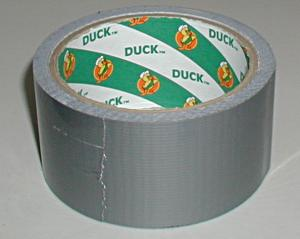
\includegraphics[scale=1.0]{pics/DuckTape.eps} \\
	\end{center}
\end{figure}
\vspace*{\fill}

\subsection{The Job of a System Administrator}
\vspace*{\fill}
\begin{figure}[hb]
	\begin{center}
		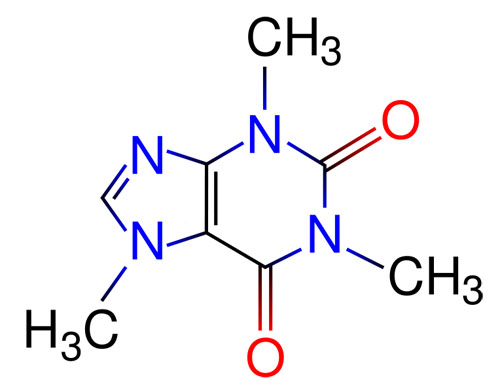
\includegraphics[scale=0.65]{pics/Caffeine_molecule.eps} \\
	\end{center}
\end{figure}
\vspace*{\fill}

\subsection{The Job of a System Administrator}
\vspace*{\fill}
\begin{figure}[hb]
	\begin{center}
		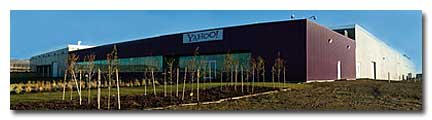
\includegraphics[scale=2.0]{pics/quincy-panorama.eps} \\
	\end{center}
\end{figure}
\vspace*{\fill}

\subsection{The Job of a System Administrator}
\vspace*{\fill}
\begin{figure}[hb]
	\begin{center}
		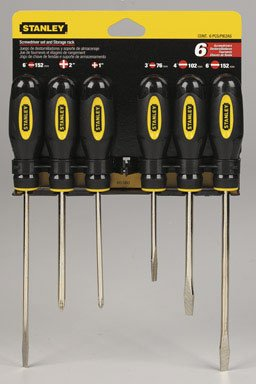
\includegraphics[scale=0.75]{pics/screwdrivers.eps} \\
	\end{center}
\end{figure}
\vspace*{\fill}

\subsection{The Job of a System Administrator}
\vspace*{\fill}
\begin{figure}[hb]
	\begin{center}
		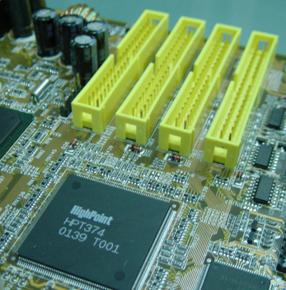
\includegraphics[scale=1.2]{pics/raid.eps} \\
	\end{center}
\end{figure}
\vspace*{\fill}

\subsection{The Job of a System Administrator}
\vspace*{\fill}
\begin{figure}[hb]
	\begin{center}
		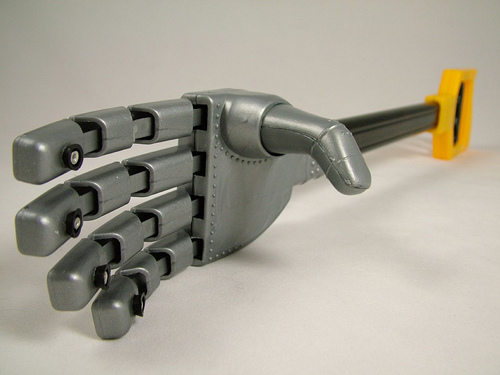
\includegraphics[scale=0.7]{pics/remote_hands.eps} \\
	\end{center}
\end{figure}
\vspace*{\fill}

\subsection{The Job of a System Administrator}
\vspace*{\fill}
\begin{figure}[hb]
	\begin{center}
		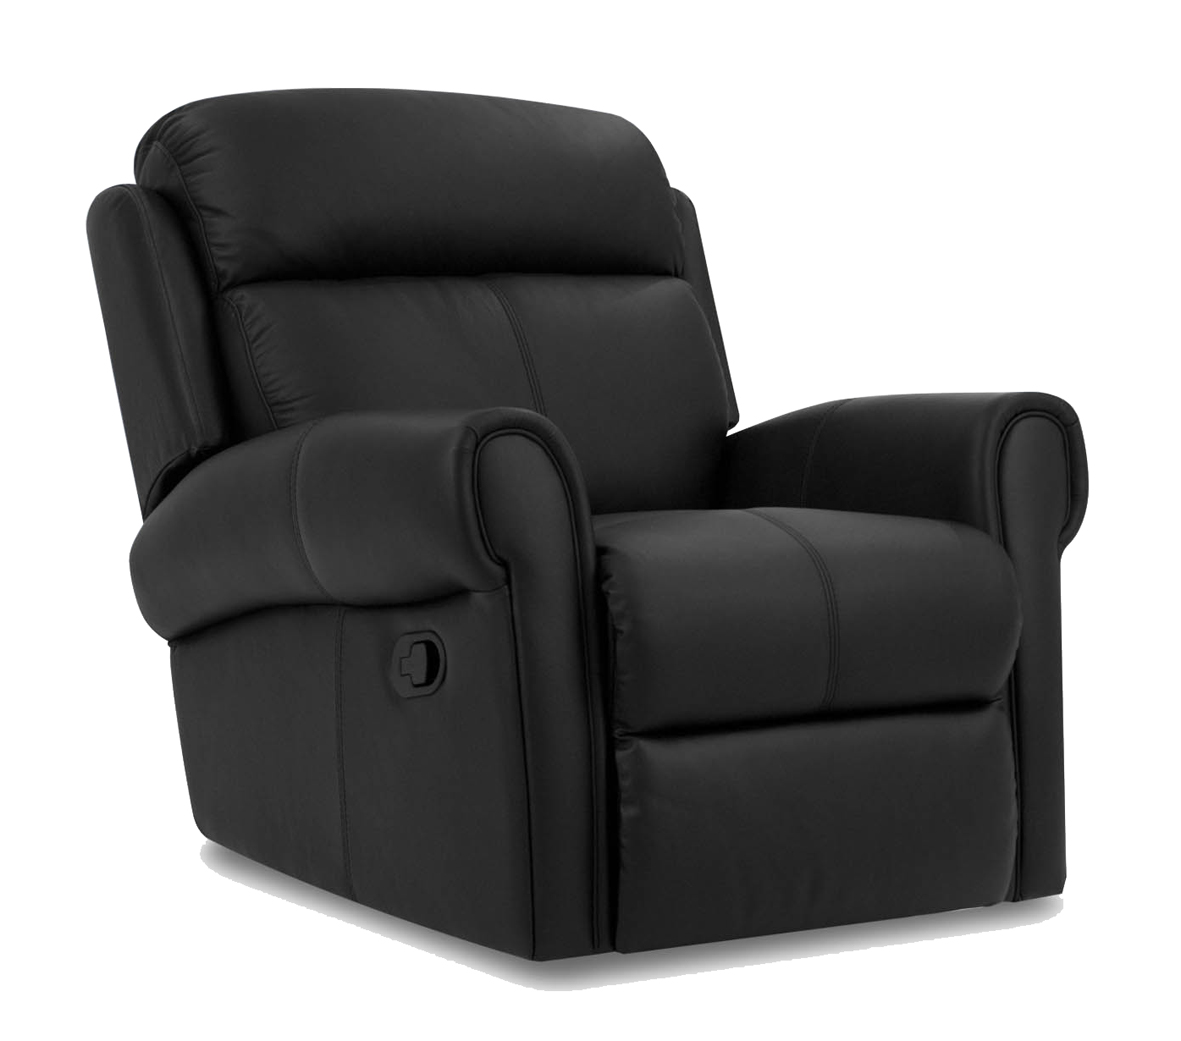
\includegraphics[scale=1.1]{pics/armchair.eps} \\
	\end{center}
\end{figure}
\vspace*{\fill}

\subsection{The Job of a System Administrator}
\vspace*{\fill}
\begin{figure}[hb]
	\begin{center}
		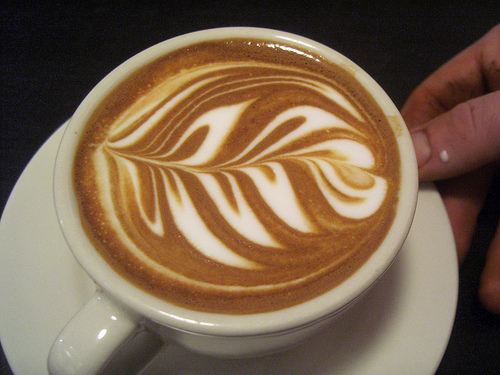
\includegraphics[scale=0.75]{pics/cappuccino.eps} \\
	\end{center}
\end{figure}
\vspace*{\fill}

\subsection{The Job of a System Administrator}
\vspace*{\fill}
\begin{figure}[hb]
	\begin{center}
		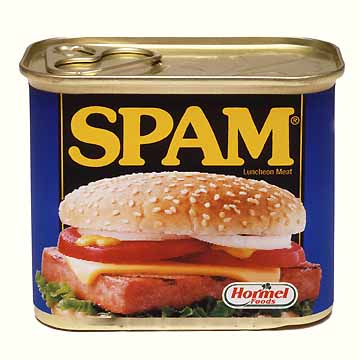
\includegraphics[scale=0.8]{pics/spam.eps} \\
	\end{center}
\end{figure}
\vspace*{\fill}

\subsection{The Job of a System Administrator}
\vspace*{\fill}
\begin{figure}[hb]
	\begin{center}
		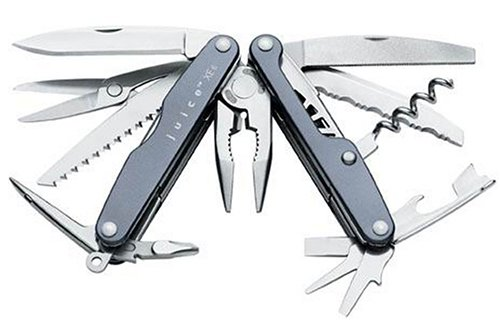
\includegraphics[scale=0.85]{pics/leatherman.eps} \\
	\end{center}
\end{figure}
\vspace*{\fill}

\subsection{The Job of a System Administrator}
\vspace*{\fill}
\begin{figure}[hb]
	\begin{center}
		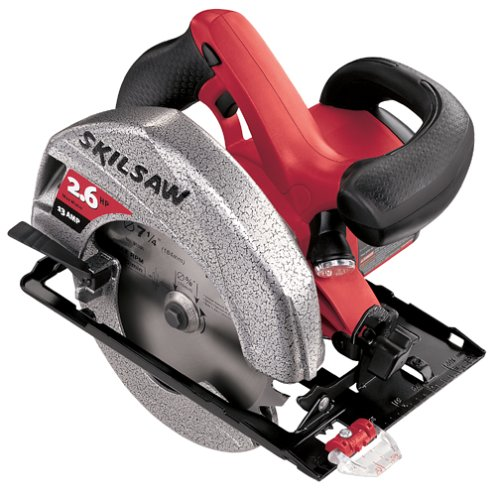
\includegraphics[scale=0.5]{pics/circularsaw.eps} \\
		\small See also: {\tt http://is.gd/WUezLL} \Normalsize
	\end{center}
\end{figure}
\vspace*{\fill}

\subsection{The Job of a System Administrator}
\vspace*{\fill}
\begin{figure}[hb]
	\begin{center}
		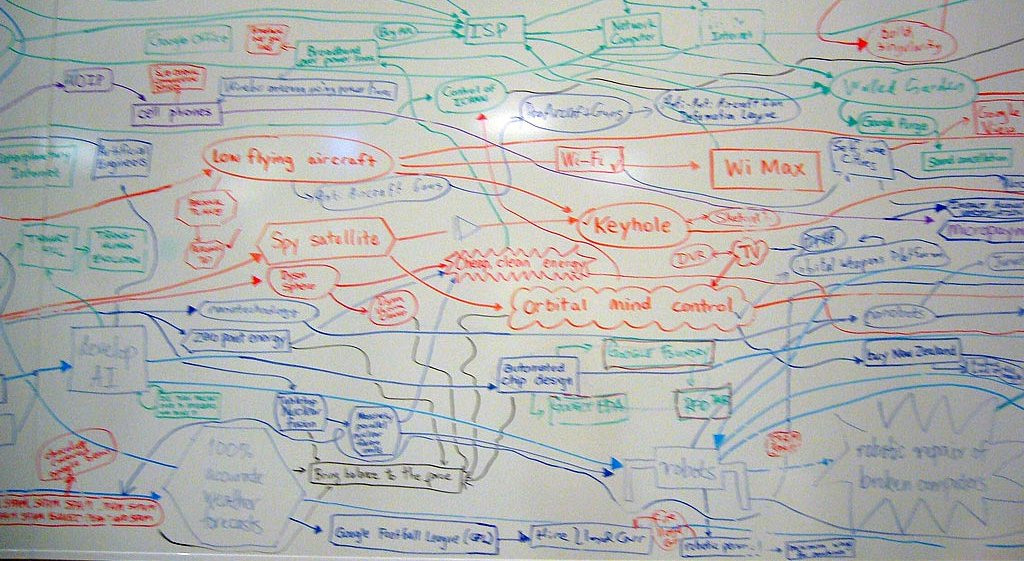
\includegraphics[scale=0.52]{pics/google_whiteboard_large.eps} \\
	\end{center}
\end{figure}
\vspace*{\fill}

\subsection{The Job of a System Administrator}
\vspace*{\fill}
\begin{figure}[hb]
	\begin{center}
		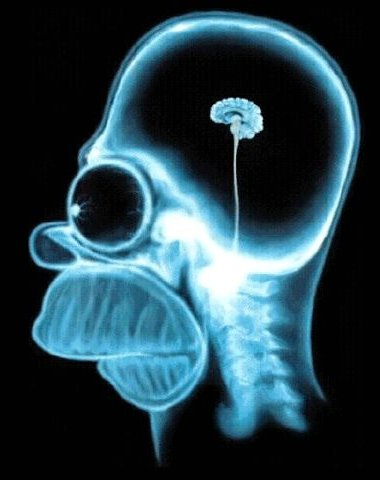
\includegraphics[scale=0.6]{pics/home-brain.eps} \\
	\end{center}
\end{figure}
\vspace*{\fill}

\subsection{The Job of a System Administrator}
What {\bf exactly} does a {\em System Administrator} do?

\subsection{The Job of a System Administrator}
What {\bf exactly} does a {\em System Administrator} do?
\begin{itemize}
	\item no precise job description
\end{itemize}

\subsection{The Job of a System Administrator}
What {\bf exactly} does a {\em System Administrator} do?
\begin{itemize}
	\item no precise job description
\end{itemize}
\begin{figure}[hb]
	\begin{center}
		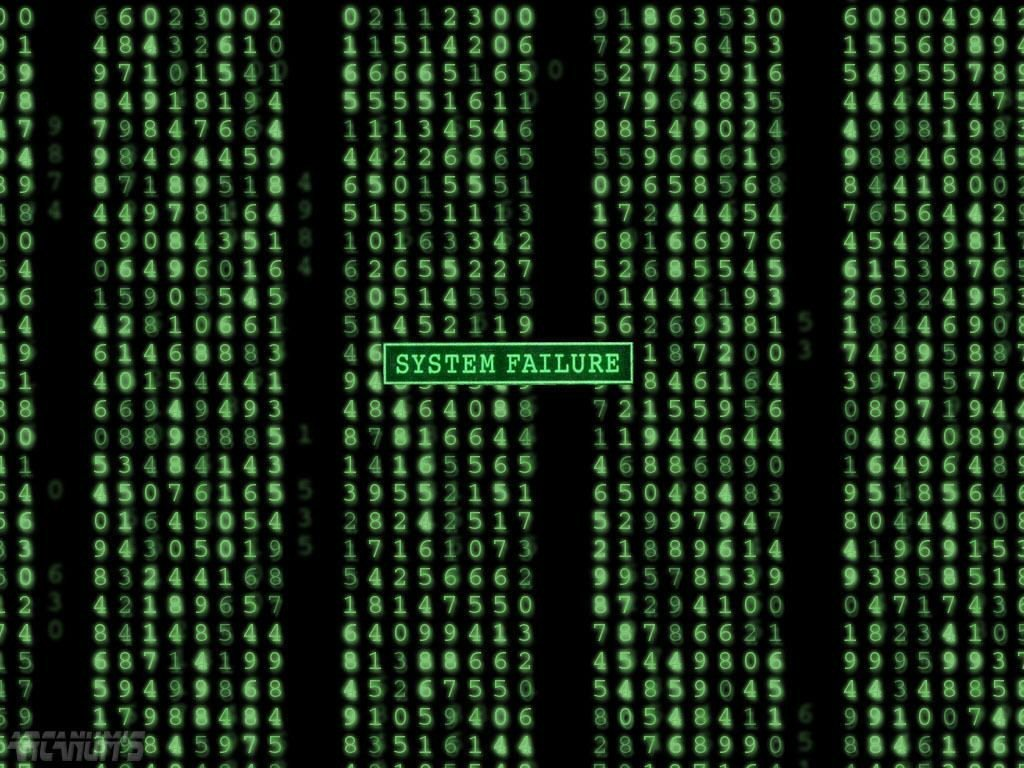
\includegraphics[scale=1.0]{pics/matrix.eps} \\
	\end{center}
\end{figure}



\subsection{The Job of a System Administrator}
What {\bf exactly} does a {\em System Administrator} do?
\begin{itemize}
	\item no precise job description
\end{itemize}
\vfill
 system administrator n.: \\
{\em one who, as a primary job function,
	manages computer and network systems on behalf of another, such as an
	employer or client.}

\subsection{The Job of a System Administrator}
What {\bf exactly} does a {\em System Administrator} do?
\begin{itemize}
	\item no precise job description
	\item often learned by experience
\end{itemize}
\vfill
system administrator n.: \\
{\em one who, as a primary job function,
	manages computer and network systems on behalf of another, such as an
	employer or client.}

\subsection{The Job of a System Administrator}
What {\bf exactly} does a {\em System Administrator} do?
\begin{itemize}
	\item no precise job description
	\item often learned by experience
	\item ``makes things run''
\end{itemize}
\vfill
system administrator n.: \\
{\em one who, as a primary job function,
	manages computer and network systems on behalf of another, such as an
	employer or client.}

\subsection{The Job of a System Administrator}
What {\bf exactly} does a {\em System Administrator} do?
\begin{itemize}
	\item no precise job description
	\item often learned by experience
	\item ``makes things run''
	\item work behind the scenes
\end{itemize}
\vfill
system administrator n.: \\
{\em one who, as a primary job function,
	manages computer and network systems on behalf of another, such as an
	employer or client.}

\subsection{The Job of a System Administrator}
What {\bf exactly} does a {\em System Administrator} do?
\begin{itemize}
	\item no precise job description
	\item often learned by experience
	\item ``makes things run''
	\item work behind the scenes
	\item often known as Operator, Network Administrator, System Programmer, System
		Manager, Service Engineer, Site Reliability Engineer etc.
\end{itemize}
\vfill
system administrator n.: \\
{\em one who, as a primary job function,
	manages computer and network systems on behalf of another, such as an
	employer or client.}

\subsection{So what is a {\em System}?}
``"A group of interacting, interrelated, or interdependent elements that
together form a complex whole.''


\subsection{So what is a {\em System}?}
``"A group of interacting, interrelated, or interdependent elements that
together form a complex whole.''
\\

In the context of this class, we generally consider {\em computer-human
systems} consisting of

\begin{itemize}
	\item the computer(s)
\end{itemize}

\subsection{So what is a {\em System}?}
``"A group of interacting, interrelated, or interdependent elements that
together form a complex whole.''
\\

In the context of this class, we generally consider {\em computer-human
systems} consisting of

\begin{itemize}
	\item the computer(s)
	\item the network
\end{itemize}

\subsection{So what is a {\em System}?}
``"A group of interacting, interrelated, or interdependent elements that
together form a complex whole.''
\\

In the context of this class, we generally consider {\em computer-human
systems} consisting of

\begin{itemize}
	\item the computer(s)
	\item the network
	\item the user(s)
\end{itemize}

\subsection{So what is a {\em System}?}
``"A group of interacting, interrelated, or interdependent elements that
together form a complex whole.''
\\

In the context of this class, we generally consider {\em computer-human
systems} consisting of

\begin{itemize}
	\item the computer(s)
	\item the network
	\item the user(s)
	\item the organization's goals and policies
\end{itemize}

\subsection{... and {\em Administration}?}
Merriam Webster:
\begin{quote}
	{\bf administer, v:} {\em to manage or supervise the execution, use, or conduct of} \\
\end{quote}


\subsection{... and {\em Administration}?}
Merriam Webster:
\begin{quote}
	{\bf administer, v:} {\em to manage or supervise the execution, use, or conduct of} \\
\end{quote}

{\em System} Administration frequently also includes other tasks such as
\begin{itemize}
	\item system design and architecture
\end{itemize}

\subsection{... and {\em Administration}?}
Merriam Webster:
\begin{quote}
	{\bf administer, v:} {\em to manage or supervise the execution, use, or conduct of} \\
\end{quote}

{\em System} Administration frequently also includes other tasks such as
\begin{itemize}
	\item system design and architecture
	\item reliability studies
\end{itemize}

\subsection{... and {\em Administration}?}
Merriam Webster:
\begin{quote}
	{\bf administer, v:} {\em to manage or supervise the execution, use, or conduct of} \\
\end{quote}


{\em System} Administration frequently also includes other tasks such as
\begin{itemize}
	\item system design and architecture
	\item reliability studies
	\item resource management
\end{itemize}

\subsection{... and {\em Administration}?}
Merriam Webster:
\begin{quote}
	{\bf administer, v:} {\em to manage or supervise the execution, use, or conduct of} \\
\end{quote}

{\em System} Administration frequently also includes other tasks such as
\begin{itemize}
	\item system design and architecture
	\item reliability studies
	\item resource management
	\item system fault diagnosis
\end{itemize}

\subsection{... and {\em Administration}?} Merriam Webster: \begin{quote} {\bf
administer, v:} {\em to manage or supervise the execution, use, or conduct of}
\\ \end{quote}

{\em System} Administration frequently also includes other tasks such as
\begin{itemize}
	\item system design and architecture
	\item reliability studies
	\item resource management
	\item system fault diagnosis
	\item ...
\end{itemize}


\subsection{... and {\em Administration}?}
Merriam Webster:
\begin{quote}
	{\bf administer, v:} {\em to manage or supervise the execution, use, or conduct of} \\
\end{quote}

{\em System} Administration frequently also includes other tasks such as
\begin{itemize}
	\item system design and architecture
	\item reliability studies
	\item resource management
	\item system fault diagnosis
	\item ...
\end{itemize}
\vspace{.5in}

...all of which my involve a fair amount of {\em software development}, {\em
programming} and {\em scripting}.

\subsection{Problem Solving}
Start with some Einstein:
\begin{quote}
{\em ``It is the aim of science to establish general rules which determine the
reciprocal connection of objects and events in time and space.''}
\end{quote}

\subsection{Problem Solving}
Start with some Einstein:
\begin{quote}
{\em ``It is the aim of science to establish general rules which determine the
reciprocal connection of objects and events in time and space.''}
\end{quote}
Add Ockham's Razor (aka the Law of Parsimony):
\begin{quote}
{\em ``Of two equivalent theories or explanations, all other things being
equal, the simpler one is to be preferred.''}
\end{quote}

\subsection{Problem Solving}
Start with some Einstein:
\begin{quote}
{\em ``It is the aim of science to establish general rules which determine the
reciprocal connection of objects and events in time and space.''}
\end{quote}
Add Ockham's Razor (aka the Law of Parsimony):
\begin{quote}
{\em ``Of two equivalent theories or explanations, all other things being
equal, the simpler one is to be preferred.''}
\end{quote}
Throw in some philosophy for good measure:
\begin{quote}
{\em Causality: For every effect, there must be a cause.}
\end{quote}

And we end up with...

\subsection{Problem Solving}
A typical task in the life of a System Administrator:

\begin{enumerate}
	\item Observe that backups are taking longer than acceptable.
	\item Consider factors that influence backups, such as
		\begin{itemize}
			\item filesystem size
			\item other activity during backup
			\item network speed and usage
			\item tape drive speed and capacity
		\end{itemize}
	\item Determine which factor to change to increase efficiency
	\item Try it out
	\item Repeat (if necessary)
\end{enumerate}

Which, of course is just...

\subsection{Problem Solving}
The {\em Scientific Method}:

\begin{enumerate}
	\item Characterization
	\item Hypothesis
	\item Prediction
	\item Experiment
	\item Repeat (if necessary)
\end{enumerate}

In other words, we continually strive to uncover the most likely explanation
for observable phenomena and influence and adjust the system following our
equally continually developing theories and goals.

\subsection{Problem Solving... in real life}
\begin{figure}[hb]
	\begin{center}
		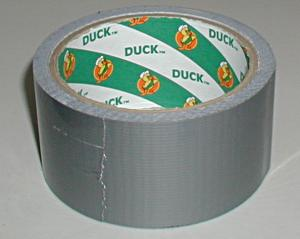
\includegraphics[scale=1.0]{pics/DuckTape.eps} \\
	\end{center}
\end{figure}

\subsection{People think the internet looks like this.}
\begin{figure}[hb]
	\begin{center}
		
\includegraphics[scale=0.7]{pics/cloud.eps} \\
	\end{center}
\end{figure}

\subsection{Or like this.}
\begin{figure}[hb]
	\begin{center}
		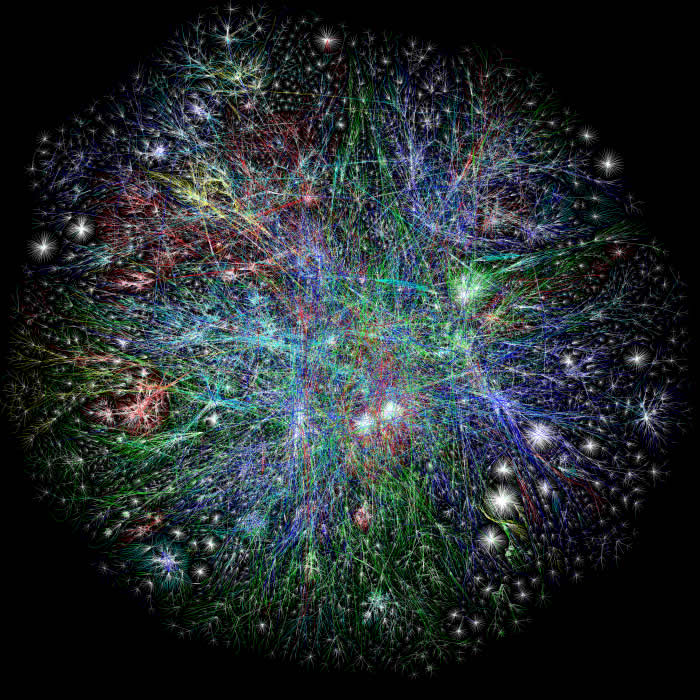
\includegraphics[scale=0.4]{pics/internet.eps} \\
	\end{center}
\end{figure}

\subsection{In reality...}
\vspace*{\fill}
\begin{center}
    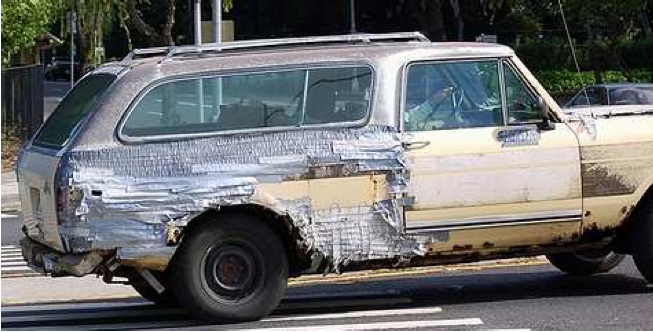
\includegraphics[scale=0.9]{pics/car-duct-tape.eps}
\end{center}
\vspace*{\fill}

\newpage
\vspace*{\fill}
\begin{center}
    \Hugesize
        Hooray! \\ [1em]
    \hspace*{5mm}
    \blueline\\
    \hspace*{5mm}\\
        5 Minute Break
\end{center}
\vspace*{\fill}

\subsection{In reality...}
\vspace*{\fill}
\begin{center}
    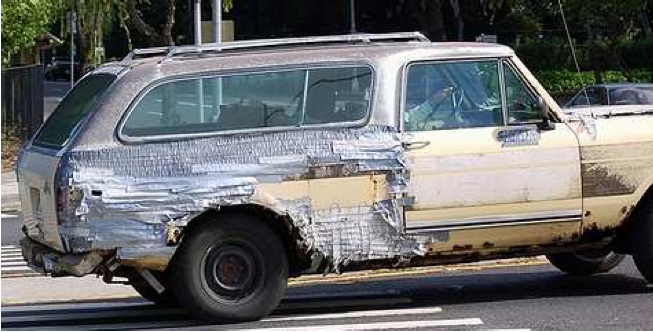
\includegraphics[scale=0.9]{pics/car-duct-tape.eps}
\end{center}
\vspace*{\fill}

\subsection{About this class}
We can only cover {\em some} of the aspects of System Administration.
\vspace*{\fill}
\begin{center}
	\includegraphics[scale=0.8]{pics/hats.eps}
\Normalsize
\end{center}
\vspace*{\fill}

\subsection{Three Pillars of Exceptional System Design}
We will give particular attention to these three core features:
\begin{itemize}
	\item Scalability
	\item Security
	\item Simplicity
\end{itemize}

\subsection{Three Pillars of Exceptional System Design: Scalability}
\vspace*{\fill}
\begin{center}
    \includegraphics[scale=0.8]{pics/donkey_too_small_for_load.eps} \\
	System Overload
\end{center}
\vspace*{\fill}

\subsection{Three Pillars of Exceptional System Design: Scalability}
\vspace*{\fill}
\begin{center}
    \includegraphics[scale=0.2]{pics/donkey_too_small_for_load.eps} \\
    \includegraphics[scale=0.4]{pics/ardennes-horse.eps} \\
	Scaling Vertically
\end{center}
\vspace*{\fill}


\subsection{Three Pillars of Exceptional System Design: Scalability}
\vspace*{\fill}
\begin{center}
    \includegraphics[scale=0.2]{pics/donkey_too_small_for_load.eps} \\
    \includegraphics[scale=0.5]{pics/vierspaenner.eps} \\
	Scaling Horizontally
\end{center}
\vspace*{\fill}

\subsection{Three Pillars of Exceptional System Design: Scalability}
\vspace*{\fill}
\begin{center}
    \includegraphics[scale=0.2]{pics/donkey_too_small_for_load.eps} \\
    \includegraphics[scale=1.1]{pics/dogcart.eps} \\
	Scaling Down
\end{center}
\vspace*{\fill}

\subsection{Three Pillars of Exceptional System Design: Security}
\vspace*{\fill}
\begin{center}
    \includegraphics[scale=1.4]{pics/usability-security.eps} \\
\end{center}
\vspace*{\fill}

\subsection{Three Pillars of Exceptional System Design: Security}
\vspace*{\fill}
\begin{center}
    \includegraphics[scale=1.0]{pics/patch-bandaid.eps} \\
\end{center}
\vspace*{\fill}

\subsection{Three Pillars of Exceptional System Design: Security}
\vspace*{\fill}
\begin{center}
    \includegraphics[scale=1.4]{pics/wrong-usability.eps} \\
\end{center}
\vspace*{\fill}

\subsection{Three Pillars of Exceptional System Design: Security}
\vspace*{\fill}
\begin{center}
    \includegraphics[scale=1.1]{pics/better-usability.eps} \\
\end{center}
\vspace*{\fill}


\subsection{Three Pillars of Exceptional System Design: Simplicity}
\vspace*{\fill}
\begin{center}
    \includegraphics[scale=0.3]{pics/kiss.eps} \\
\end{center}
\vspace*{\fill}

\subsection{Three Pillars of Exceptional System Design: Simplicity}
\vspace*{\fill}
\begin{center}
    \includegraphics[scale=1.2]{pics/lego-block.eps} \\
\end{center}
\vspace*{\fill}

\subsection{Three Pillars of Exceptional System Design: Simplicity}
\vspace*{\fill}
\begin{center}
    \includegraphics[scale=0.1]{pics/millennium-falcon.eps} \\
\end{center}
\vspace*{\fill}







\subsection{About this class}
Suggested Reading:
\begin{itemize}
	\item ``Essential System Administration'', 3rd Edition, by \AE leen
		Frisch
	\item ``Unix System Administration Handbook'', 3rd Edition, by Evi Nemeth
	\item ``Principles of Network and System Administration'', by Mark Burgess
	\item ``Analytical Network and System Administration'', by Mark Burgess
	\item ``The Practice of System and Network Administration'', by Thomas
		A. Limoncelli \& Christine Hogan
\end{itemize}
\addvspace{.5in}
Grading:
\begin{itemize}
	\item a few pop quizzes, worth 20 points each.
	\item a number of homework assignments of varying weight
	\item 1 presentation/paper, worth 100 points
	\item no curve
\end{itemize}

\subsection{Syllabus}
%Topics:
\begin{itemize}
	\item 2012-01-23: Introduction, Overview, UNIX history and basics
	\item 2012-01-30: Filesystems and Disks
	\item 2012-02-06: Software Installation Concepts
	\item 2012-02-13: User Management, multi-user basics
	\item 2012-02-21: Automating Administrative Tasks
	\item 2012-02-27: Backup and Disaster Recovery
	\item 2012-03-05: Networking
	\item 2012-03-12: Spring Break
	\item 2012-03-19: Popular services (DNS, SMTP)
	\item 2012-03-26: Popular services (HTTP, SNMP, SSH)
	\item 2012-04-02: System Security
	\item 2012-04-09 -- 2011-04-30: AMA / Misc. topics and presentations
\end{itemize}

\subsection{Syllabus}
Miscellaneous topics and presentations may include:
\begin{itemize}
	\item large scale logging
	\item heterogenous networks / multiple OS
	\item automated installation
	\item configuration management
	\item server room basics, cooling issues, racking etc.
	\item clustering
	\item spam
	\item \ldots
\end{itemize}

\subsection{Questions, Answers, Chatter...}
\begin{itemize}
	\item 10 minutes of Ask Me Anything / current events at the beginning of the class \\
		\small that does {\em not} mean you can come 10 minutes late \Normalsize
	\\

	\item course website, syllabus, assignments, course material:\\
		\verb+http://www.cs.stevens.edu/~jschauma/615/+
	\\

	\item discussions and announcements:
		\verb+https://lists.stevens.edu/cgi-bin/mailman/listinfo/cs615asa+
	\\

	\item who knows what: \verb+http://twitter.com/cs615asa+
\end{itemize}

\newpage
\vspace*{\fill}
\begin{center}
    \Hugesize
        UNIX \\ [1em]
    \hspace*{5mm}
    \blueline\\
    \hspace*{5mm}\\
        History and Basics
\end{center}
\vspace*{\fill}


\subsection{UNIX history}
\begin{itemize}
	\item Originally developed in 1969 at Bell Labs by Ken Thompson
		and Dennis Ritchie.

\begin{figure}[hb]
	\begin{center}
		\includegraphics[scale=6.0]{pics/pdp11.eps} \\
	\end{center}
\end{figure}

	\item 1974: Thompson, Joy, Haley and students at Berkeley develop
		the Berkeley Software Distribution (BSD) of UNIX
\end{itemize}

\subsection{UNIX Philosophy}
\begin{figure}[hb]
	\begin{center}
		\includegraphics[scale=0.5]{pics/MagrittePipe.eps} \\
	\end{center}
\end{figure}
\begin{center}
	{\bf Do one thing and do it well.}
\end{center}




\subsection{UNIX history}
\begin{itemize}
	\item 1978: ``Version 7 Unix'' released; AT\&T licenses ``System III'' commercially
	\item BSD and ``System V'' become the main directions
	\item 1991: BSD re-written almost entirely from scratch to allow
		redistribution without AT\&T license as Networking Release 2 ({\em Net/2}),
		spawning BSD/OS (commercial) and 386BSD, from which both
		FreeBSD and NetBSD were derived in 1993
	\item 1992: ``Unix Systems Laboratories'' (USL) sues BSDI and UC Berkely \\
	      \small {\tt https://en.wikipedia.org/wiki/USL\_v.\_BSDi} \Normalsize
	\item settlement leads to 4.4BSD-Lite, which feeds back into
		FreeBSD and NetBSD
\end{itemize}

\subsection{UNIX history}
\begin{itemize}
	\item 1983: the GNU project started to develop another Unix-like operating system
	\item the Linux kernel is released in 1991 and becomes GNU's
		kernel in 1992
	\\

	\item 2001: Mac OS X is released, based on Darwin, which incorporates NeXTSTEP (Mach
		kernel + BSD userland), FreeBSD, NetBSD
\end{itemize}

\subsection{UNIX history}
\vspace*{\fill}
\begin{figure}[hb]
	\begin{center}
		\includegraphics[scale=0.5]{pics/unix_history.eps} \\
	\end{center}
\end{figure}
\vspace*{\fill}

\subsection{Some OS versions}
How many Unix variations/derivatives can you name?

\subsection{Some OS versions}
Some Operating Systems variations you may encounter:
\\

\vspace{.5in}
\begin{center}
\begin{tabular}{ c c c c }
	A/UX & AIX & IRIX & Darwin \\
	GNU/Hurd & Digital Unix & DragonFly BSD & FreeBSD \\
	HP-UX & Mac OS X & IOS & JunOS \\
	MS Windows & zOS & Minix & NetBSD \\
	Ultrix & OpenBSD & OS/390 Unix & OSF/1 \\
	Plan 9 & Inferno & QNX RTOS & SCO UnixWare \\
	SCO Xenix & Solaris & SunOS & Tru64 Unix \\
\end{tabular}
\\
\vspace{.5in}
	Various Linux flavors
\end{center}

\subsection{UNIX Basics}
\vspace*{\fill}
\begin{center}
	\includegraphics[scale=0.6]{pics/System-Call-and-Library-Function.eps} \\
\end{center}
\vspace*{\fill}

%\subsection{UNIX Basics}
%\\
%
%\begin{center}
%	\includegraphics[scale=0.7]{pics/kernel-programs.eps} \\
%\end{center}

\subsection{UNIX Basics}
\vspace*{\fill}
\begin{center}
	\includegraphics[scale=0.7]{pics/unix-parts.eps} \\
\end{center}
\vspace*{\fill}


\subsection{UNIX Basics}
The OS is divided into
\begin{itemize}
	\item kernel
	\item shell
	\item tools \& applications
\end{itemize}
\addvspace{.5in}
Basic UNIX features:
\begin{itemize}
	\item multitasking
	\item multiuser
	\item portability
	\item networking capabilities
\end{itemize}

\subsection{UNIX Basics}
These features necessitate/result in:
\begin{itemize}
	\item multi-user concepts
		\begin{itemize}
			\item user privileges
			\item file permissions
			\item process ownership and priorities
			\item communication with users
			\item disk quotas
		\end{itemize}
	\item superuser account
		\begin{itemize}
			\item unrestricted access for superuser
			\item requires strong authentication
		\end{itemize}
	\item security considerations
		\begin{itemize}
			\item protect users data
			\item protect communication
			\item protect superuser account
		\end{itemize}
\end{itemize}

\subsection{Homework}
\begin{itemize}
	\item General:
		\begin{itemize}
			\item make sure you have access to \verb+lab.cs.stevens.edu+
			\item subscribe to \verb+cs615asa@lists.stevens.edu+
		\end{itemize}
		\vspace{.5in}

	\item Research Cloud Computing:
		\begin{itemize}
			\item \verb+https://en.wikipedia.org/wiki/Cloud_computing+
			\item \verb+https://en.wikipedia.org/wiki/Amazon_Elastic_Compute_Cloud+
		\end{itemize}
		\vspace{.5in}

	\item Create an Amazon EC2 account:
		\begin{itemize}
			\item \verb+https://aws.amazon.com/ec2/+
		\end{itemize}
\end{itemize}


\subsection{Reading}
System Administrator Job Description
\begin{itemize}
	\item Frisch: Preface; Limoncelli \& Hogan: Preface, 26; Nemeth: 1;
		Burgess: 1, 2, 14
	\item \verb+http://www.sage.org/pubs/22_jobs/+
\end{itemize}

UNIX history:
\begin{itemize}
	\item \verb+http://www.bell-labs.com/history/unix/+
	\item \verb+http://www.futuretech.blinkenlights.nl/admin/day1a.html+
	\item \verb+http://www.levenez.com/unix/+
	\item \verb+https://en.wikipedia.org/wiki/Operating_system+
\end{itemize}

UNIX basics:
\begin{itemize}
	\item chmod(1), chown(1), ls(1)
	\item intro(1), login(1), passwd(5)
	\item su(1), sudo(8)
\end{itemize}

%\nocite{*}
%\bibliographystyle{plain}
%\bibliography{slides}

\end{document}
